\documentclass{article}
\usepackage[utf8]{inputenc}
\usepackage{polski}
\usepackage{graphicx}
\usepackage[margin= 3cm]{geometry}


\title{Wskaźnik MACD}
\author{Piotr Pesta}
\date{Marzec 2022}
\setlength{\parindent}{20pt}
\graphicspath{{./Graphs/}}

\begin{document}
\maketitle

\section{Wstęp}

    Celem projektu było zaimplementowanie wskaźnika MACD, który pozwala na podstawie analizy danych z przeszłości
    wyznaczać momenty kupna i sprzedarzy udziałów.
    Implementacji dokonałem w języku Python z wykorzystaniem bibliotek pandas oraz matplotlib.
    Dane wejściowe to plik .csv zawierający informacje o cenach udziałów z konkretnych dni. 
    Jako wartość udziałów w danym dniu wykorzystałem cenę zamknięcia z tego dnia.

\section{Analiza zadania}

    W celu określenia na podstawie wskaźnika MACD momentów kupna i sprzedaży akcji należy obliczyć
    dwie średnie kroczące:
    \begin{itemize}
        \item krótkookresową - w zadaniu jest to 12 okresów
        \item długookresową - 26 okresów
    \end{itemize}

    Można do 

\section{Przykład działania}


   \noindent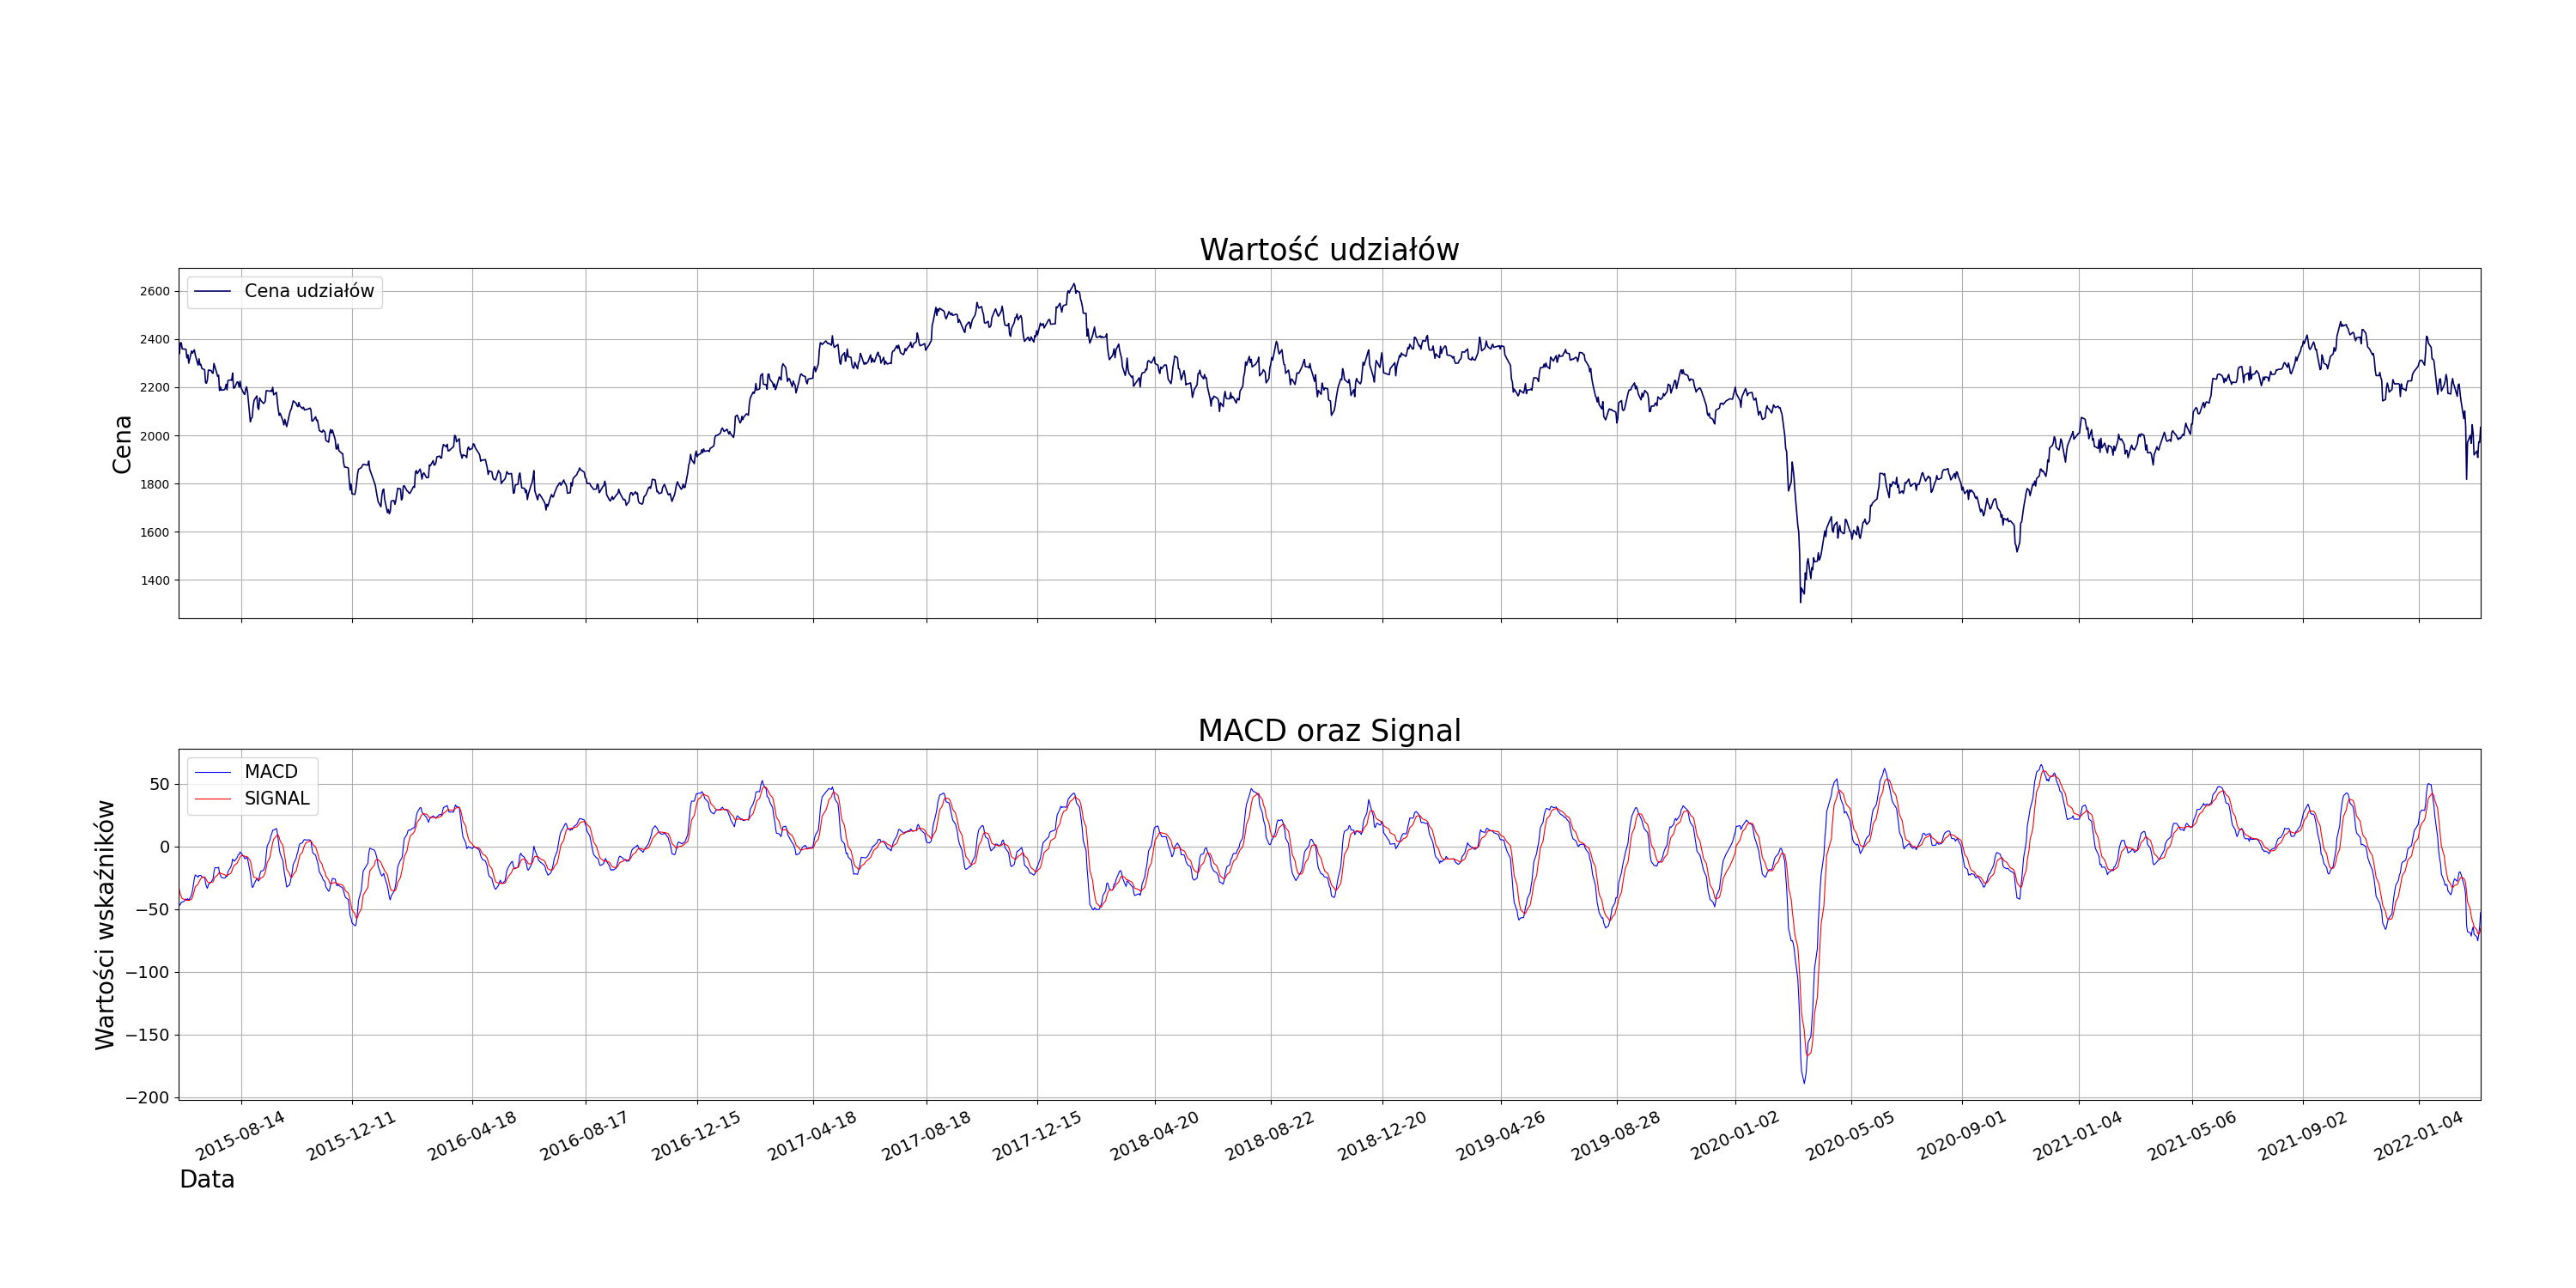
\includegraphics[width=\textwidth]{WIG20}

\section{Analiza przydatności MACD do inwestowania}

    Tutaj analiza algorytmu do inwestowania

\end{document}